\section{Sprint Report}
% stories completed, progress report (e.g., through a burndown chart), next sprint

\subsection{Current Sprint}

The following stories was completed as planed at the start of the sprint:
\begin{itemize}
    \item Create code that can save the translated LinkedIn data to the Leapkit Database.
    \item Setup Jenkins environment
    \item Implement basic match making algorithm ready for iterative developement/extensions
    \item Create test suite for the code generated in the previous sprint.
\end{itemize}

\begin{figure}[!ht]
    \centering
    \begin{subfigure}[b]{0.5\textwidth}
        \scalebox{.6}{\begin{tikzpicture}

% horizontal axis
    \draw[->] (0,0) -- (8,0) node[anchor=north] {\emph{Day}};
% labels
    \draw   (0,0) node[anchor=north] {0}
            (1,0) node[anchor=north] {1}
            (2,0) node[anchor=north] {2}
            (3,0) node[anchor=north] {3}
            (4,0) node[anchor=north] {4}
            (5,0) node[anchor=north] {5}
            (6,0) node[anchor=north] {6}
            (7,0) node[anchor=north] {7};

% vertical axis
    \draw[->] (0,0) -- (0,8) node[anchor=east] {\emph{Points remaining}};
% labels
    \draw   (0,1) node[anchor=east] {3}
            (0,2) node[anchor=east] {5.5}
            (0,3) node[anchor=east] {8}
            (0,4) node[anchor=east] {10.5}
            (0,5) node[anchor=east] {12}
            (0,6) node[anchor=east] {15.5}
            (0,7) node[anchor=east] {18};

% projected 
    \draw[thick, dotted, red] (0,7) -- (7,0);

% actual
    \draw[thick, blue] (0,7) -- (1,6.5) -- (2,6.0) -- (3,4) -- (4,2.5) -- (5,2.5) -- (6,1); 
   
% legend
    \begin{scope}[shift={(4,4)}] 
        \draw[thick, dotted, red] (0,0) -- (0.5,0) 
            node[black, right]{Projected Sprint};
        \draw[thick, blue, yshift=\baselineskip] (0,0) -- 
            plot[] (0.25,0) -- (0.5,0)
            node[black, right]{Actual Sprint};
    \end{scope}
\end{tikzpicture}
}
        \caption{Burndown of the current sprint}
        \label{fig:burndownSprint}
    \end{subfigure}%
    \begin{subfigure}[b]{0.5\textwidth}
        \scalebox{.7}{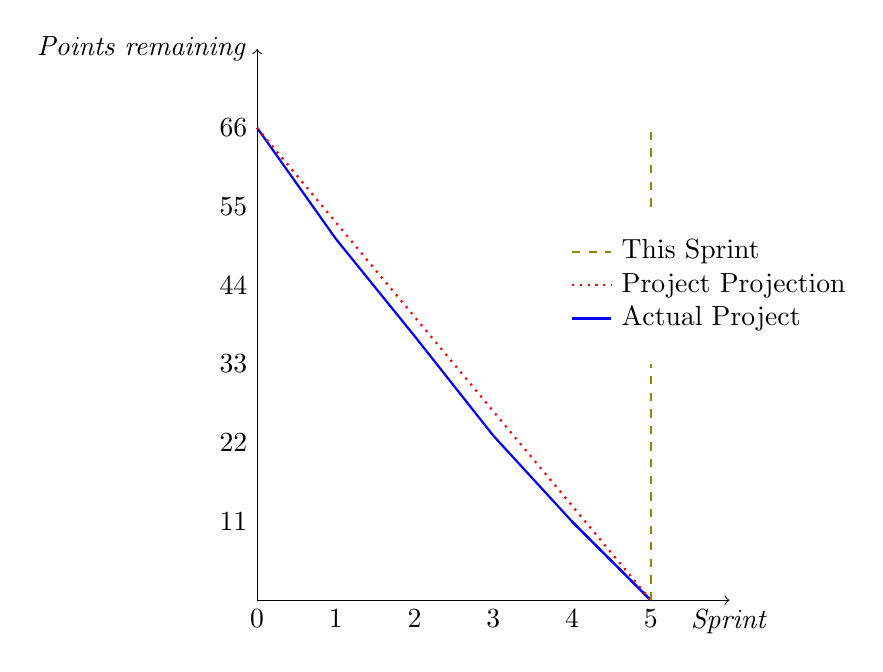
\begin{tikzpicture}

% horizontal axis
    \draw[->] (0,0) -- (6,0) node[anchor=north] {\emph{Sprint}};
% labels
    \draw   (0,0) node[anchor=north] {0}
            (1,0) node[anchor=north] {1}
            (2,0) node[anchor=north] {2}
            (3,0) node[anchor=north] {3}
            (4,0) node[anchor=north] {4}
            (5,0) node[anchor=north] {5};

% vertical axis
    \draw[->] (0,0) -- (0,7) node[anchor=east] {\emph{Points remaining}};
% labels
    \draw   (0,1) node[anchor=east] {11}
            (0,2) node[anchor=east] {22}
            (0,3) node[anchor=east] {33}
            (0,4) node[anchor=east] {44}
            (0,5) node[anchor=east] {55}
            (0,6) node[anchor=east] {66};
% actual
    \draw[thick, blue] (0,6) -- (1,4.59) -- (2,3.355) -- (3,2.09)-- (4,1.00) -- (5,0);
% actual projected
    \draw[thick, dashed, blue] (4,1.00) -- (5,0);

% projected 
    \draw[thick, dotted, red] (0,6) -- (5,0);


% current sprint 
    \draw[thick, dashed, olive] (5,0) -- (5,3);
    \draw[thick, dashed, olive] (5,5) -- (5,6);


    
\begin{scope}[shift={(4,4)}] 
    \draw[thick, dotted, red] (0,0) -- (0.5,0) 
        node[black, right]{Project Projection};
    \draw[thick, blue, yshift=\baselineskip * - 1] (0,0) -- (0.5,0)
        node[black, right]{Actual Project};
    \draw[thick, dashed, olive, yshift=\baselineskip] (0,0) -- (0.5,0)
        node[black, right]{This Sprint};
\end{scope}

\end{tikzpicture}
}
        \caption{Burndown of the project}
        \label{fig:burndownProject}
    \end{subfigure}
    \caption{Burndown charts}
\end{figure}

\subsection{Next Sprint}
Next sprint will focus on integration of the current into the Leapkit solution. After this integration, the matchmaking algorithm can iteratively be expanded and CI will be the focus point. The remaining backlog items can be seen in Figure \ref{fig:backlog}.
\begin{itemize}
\item Finish database design and implementation
\item Integrate LinkedIn redirection and extraction
\item Integrate database solution
\item Integrate match making solution
\item Further expansion on match making algorithm
\end{itemize}

\graphicc{0.4}{img/backlog.png}{The current project backlog.}{fig:backlog}